

\tikzset{every picture/.style={line width=0.75pt}} %set default line width to 0.75pt        

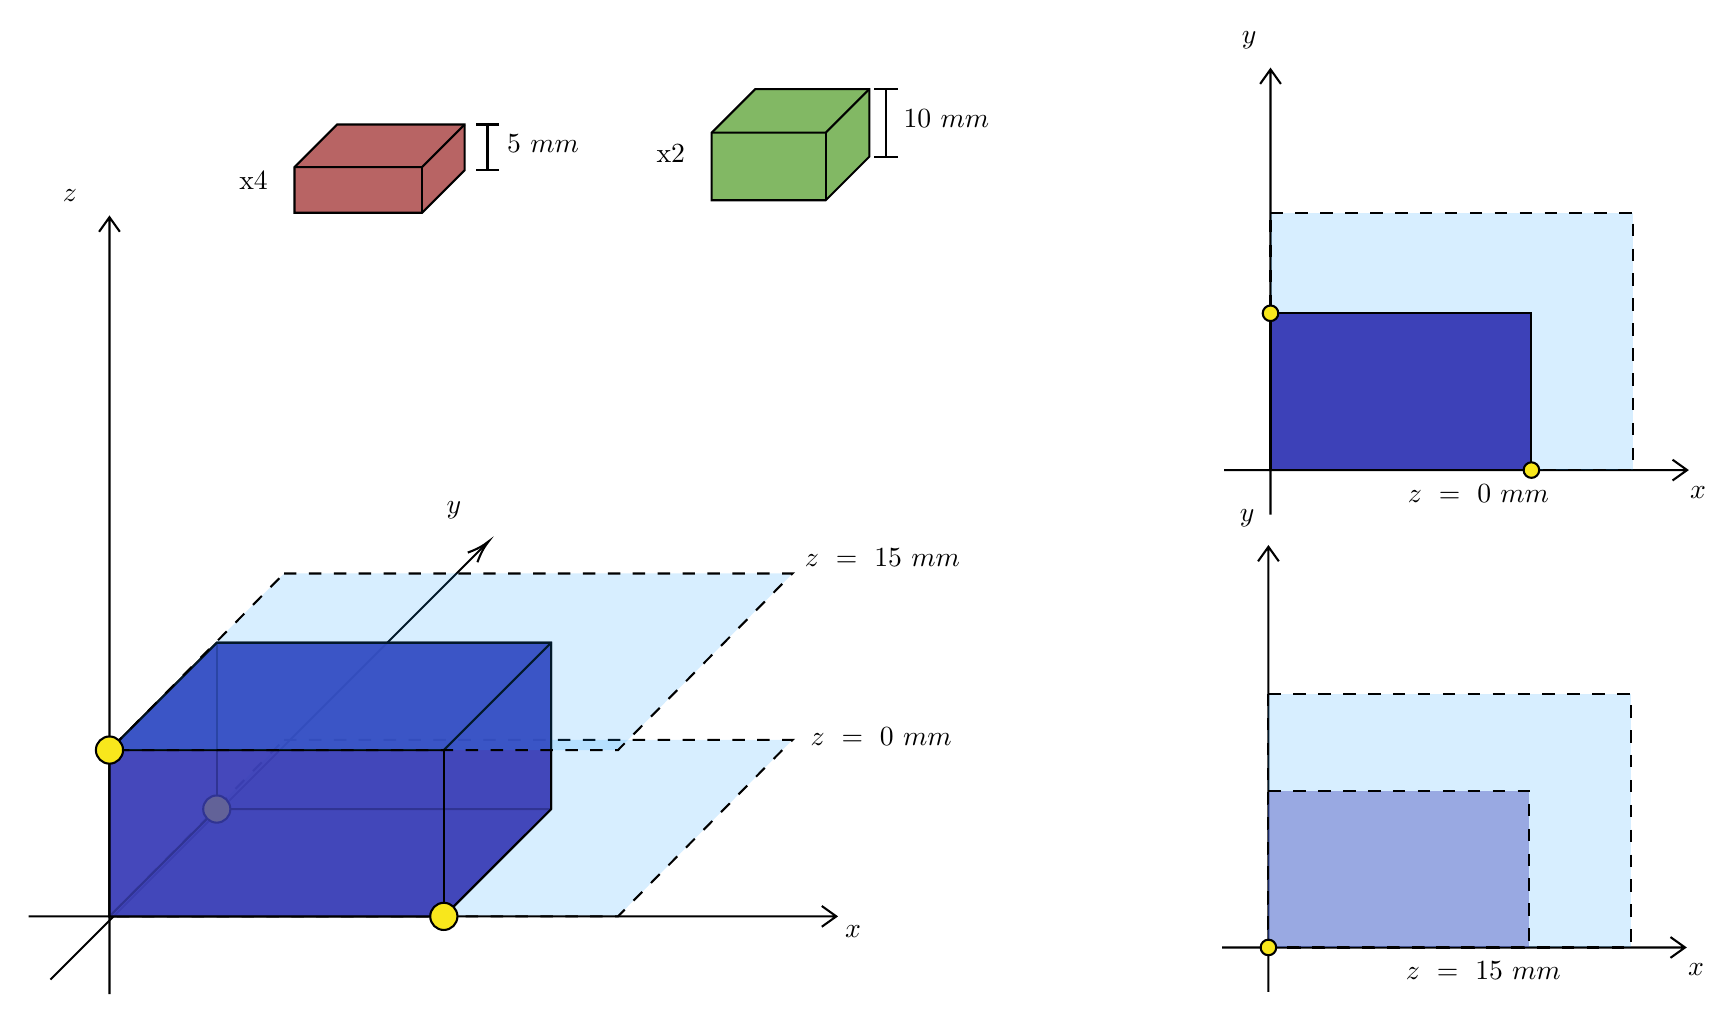
\begin{tikzpicture}[x=0.75pt,y=0.75pt,yscale=-1,xscale=1]
%uncomment if require: \path (0,526); %set diagram left start at 0, and has height of 526

%Shape: Parallelogram [id:dp4222597826124894] 
\draw  [fill={rgb, 255:red, 17; green, 154; blue, 255 }  ,fill opacity=0.17 ][dash pattern={on 4.5pt off 4.5pt}] (152,386) -- (397,386) -- (312.91,471.07) -- (67.91,471.07) -- cycle ;
%Shape: Axis 2D [id:dp7995244616027828] 
\draw  (29,471.07) -- (418.11,471.07)(67.91,134.22) -- (67.91,508.5) (411.11,466.07) -- (418.11,471.07) -- (411.11,476.07) (62.91,141.22) -- (67.91,134.22) -- (72.91,141.22)  ;
%Straight Lines [id:da046160894031782584] 
\draw    (39.47,501.52) -- (249.19,291.8) ;
\draw [shift={(250.6,290.39)}, rotate = 135] [color={rgb, 255:red, 0; green, 0; blue, 0 }  ][line width=0.75]    (10.93,-3.29) .. controls (6.95,-1.4) and (3.31,-0.3) .. (0,0) .. controls (3.31,0.3) and (6.95,1.4) .. (10.93,3.29)   ;
%Shape: Axis 2D [id:dp5764035659192752] 
\draw  (605,256.05) -- (828,256.05)(627.3,63) -- (627.3,277.5) (821,251.05) -- (828,256.05) -- (821,261.05) (622.3,70) -- (627.3,63) -- (632.3,70)  ;
%Shape: Rectangle [id:dp570599008690165] 
\draw  [fill={rgb, 255:red, 17; green, 154; blue, 255 }  ,fill opacity=0.17 ][dash pattern={on 4.5pt off 4.5pt}] (627.3,132) -- (802,132) -- (802,256.05) -- (627.3,256.05) -- cycle ;
%Shape: Cube [id:dp4526535692065705] 
\draw  [fill={rgb, 255:red, 184; green, 100; blue, 100 }  ,fill opacity=1 ] (157.05,110.05) -- (177.55,89.55) -- (239.05,89.55) -- (239.05,111.55) -- (218.55,132.05) -- (157.05,132.05) -- cycle ; \draw   (239.05,89.55) -- (218.55,110.05) -- (157.05,110.05) ; \draw   (218.55,110.05) -- (218.55,132.05) ;
%Shape: Cube [id:dp8554028533817293] 
\draw  [fill={rgb, 255:red, 130; green, 184; blue, 100 }  ,fill opacity=1 ] (358.05,93.5) -- (379.05,72.5) -- (434,72.5) -- (434,105.05) -- (413,126.05) -- (358.05,126.05) -- cycle ; \draw   (434,72.5) -- (413,93.5) -- (358.05,93.5) ; \draw   (413,93.5) -- (413,126.05) ;
%Straight Lines [id:da7979465991315938] 
\draw    (250.05,89.55) -- (250.05,111.55) ;
\draw [shift={(250.05,111.55)}, rotate = 270] [color={rgb, 255:red, 0; green, 0; blue, 0 }  ][line width=0.75]    (0,5.59) -- (0,-5.59)   ;
\draw [shift={(250.05,89.55)}, rotate = 270] [color={rgb, 255:red, 0; green, 0; blue, 0 }  ][line width=0.75]    (0,5.59) -- (0,-5.59)   ;
%Straight Lines [id:da892034196138813] 
\draw    (442,72.5) -- (442,105.05) ;
\draw [shift={(442,105.05)}, rotate = 270] [color={rgb, 255:red, 0; green, 0; blue, 0 }  ][line width=0.75]    (0,5.59) -- (0,-5.59)   ;
\draw [shift={(442,72.5)}, rotate = 270] [color={rgb, 255:red, 0; green, 0; blue, 0 }  ][line width=0.75]    (0,5.59) -- (0,-5.59)   ;
%Shape: Cube [id:dp048406160308493096] 
\draw  [fill={rgb, 255:red, 61; green, 65; blue, 184 }  ,fill opacity=0.8 ] (280.7,419.38) -- (229,471.07) -- (67.91,471.07) -- (67.91,390.94) -- (119.61,339.25) -- (280.7,339.25) -- cycle ; \draw   (67.91,471.07) -- (119.61,419.38) -- (280.7,419.38) ; \draw   (119.61,419.38) -- (119.61,339.25) ;
%Shape: Ellipse [id:dp38811273699393234] 
\draw  [fill={rgb, 255:red, 248; green, 231; blue, 28 }  ,fill opacity=1 ] (113.06,419.38) .. controls (113.06,415.76) and (115.99,412.83) .. (119.61,412.83) .. controls (123.22,412.83) and (126.15,415.76) .. (126.15,419.38) .. controls (126.15,422.99) and (123.22,425.92) .. (119.61,425.92) .. controls (115.99,425.92) and (113.06,422.99) .. (113.06,419.38) -- cycle ;
%Shape: Cube [id:dp6175116010805962] 
\draw  [fill={rgb, 255:red, 61; green, 65; blue, 184 }  ,fill opacity=0.8 ] (67.91,390.94) -- (119.61,339.25) -- (280.7,339.25) -- (280.7,419.38) -- (229,471.07) -- (67.91,471.07) -- cycle ; \draw   (280.7,339.25) -- (229,390.94) -- (67.91,390.94) ; \draw   (229,390.94) -- (229,471.07) ;
%Shape: Ellipse [id:dp8509879472929486] 
\draw  [fill={rgb, 255:red, 248; green, 231; blue, 28 }  ,fill opacity=1 ] (222.46,471.07) .. controls (222.46,467.46) and (225.39,464.53) .. (229,464.53) .. controls (232.62,464.53) and (235.55,467.46) .. (235.55,471.07) .. controls (235.55,474.69) and (232.62,477.62) .. (229,477.62) .. controls (225.39,477.62) and (222.46,474.69) .. (222.46,471.07) -- cycle ;
%Shape: Axis 2D [id:dp48062019416570856] 
\draw  (604,486.05) -- (827,486.05)(626.3,293) -- (626.3,507.5) (820,481.05) -- (827,486.05) -- (820,491.05) (621.3,300) -- (626.3,293) -- (631.3,300)  ;
%Shape: Rectangle [id:dp2573254178626563] 
\draw  [fill={rgb, 255:red, 17; green, 154; blue, 255 }  ,fill opacity=0.17 ][dash pattern={on 4.5pt off 4.5pt}] (626.3,364) -- (801,364) -- (801,486.05) -- (626.3,486.05) -- cycle ;
%Shape: Rectangle [id:dp8530743639576063] 
\draw  [fill={rgb, 255:red, 61; green, 65; blue, 184 }  ,fill opacity=1 ] (627.3,180.5) -- (753,180.5) -- (753,256.05) -- (627.3,256.05) -- cycle ;
%Shape: Circle [id:dp9590370044899046] 
\draw  [fill={rgb, 255:red, 248; green, 231; blue, 28 }  ,fill opacity=1 ] (623.55,180.5) .. controls (623.55,178.43) and (625.23,176.75) .. (627.3,176.75) .. controls (629.37,176.75) and (631.05,178.43) .. (631.05,180.5) .. controls (631.05,182.57) and (629.37,184.25) .. (627.3,184.25) .. controls (625.23,184.25) and (623.55,182.57) .. (623.55,180.5) -- cycle ;
%Shape: Circle [id:dp7919472039444115] 
\draw  [fill={rgb, 255:red, 248; green, 231; blue, 28 }  ,fill opacity=1 ] (749.25,256.05) .. controls (749.25,253.98) and (750.93,252.3) .. (753,252.3) .. controls (755.07,252.3) and (756.75,253.98) .. (756.75,256.05) .. controls (756.75,258.12) and (755.07,259.8) .. (753,259.8) .. controls (750.93,259.8) and (749.25,258.12) .. (749.25,256.05) -- cycle ;
%Shape: Rectangle [id:dp2993308124270544] 
\draw  [fill={rgb, 255:red, 61; green, 65; blue, 184 }  ,fill opacity=0.4 ][dash pattern={on 4.5pt off 4.5pt}] (626.3,410.5) -- (752,410.5) -- (752,486.05) -- (626.3,486.05) -- cycle ;
%Shape: Circle [id:dp16199792658724443] 
\draw  [fill={rgb, 255:red, 248; green, 231; blue, 28 }  ,fill opacity=1 ] (622.55,486.05) .. controls (622.55,483.98) and (624.23,482.3) .. (626.3,482.3) .. controls (628.37,482.3) and (630.05,483.98) .. (630.05,486.05) .. controls (630.05,488.12) and (628.37,489.8) .. (626.3,489.8) .. controls (624.23,489.8) and (622.55,488.12) .. (622.55,486.05) -- cycle ;
%Shape: Parallelogram [id:dp1306220090712341] 
\draw  [fill={rgb, 255:red, 17; green, 154; blue, 255 }  ,fill opacity=0.17 ][dash pattern={on 4.5pt off 4.5pt}] (152,305.87) -- (397,305.87) -- (312.91,390.94) -- (67.91,390.94) -- cycle ;
%Shape: Ellipse [id:dp7884999653092057] 
\draw  [fill={rgb, 255:red, 248; green, 231; blue, 28 }  ,fill opacity=1 ] (61.37,390.94) .. controls (61.37,387.33) and (64.3,384.4) .. (67.91,384.4) .. controls (71.52,384.4) and (74.45,387.33) .. (74.45,390.94) .. controls (74.45,394.56) and (71.52,397.49) .. (67.91,397.49) .. controls (64.3,397.49) and (61.37,394.56) .. (61.37,390.94) -- cycle ;

% Text Node
\draw (228.9,269.7) node [anchor=north west][inner sep=0.75pt]    {$y$};
% Text Node
\draw (420.84,473.85) node [anchor=north west][inner sep=0.75pt]    {$x$};
% Text Node
\draw (43.94,119.64) node [anchor=north west][inner sep=0.75pt]    {$z$};
% Text Node
\draw (828,262.4) node [anchor=north west][inner sep=0.75pt]    {$x$};
% Text Node
\draw (612,43.4) node [anchor=north west][inner sep=0.75pt]    {$y$};
% Text Node
\draw (692,261.4) node [anchor=north west][inner sep=0.75pt]    {$z\ =\ 0\ mm$};
% Text Node
\draw (330,98) node [anchor=north west][inner sep=0.75pt]   [align=left] {x2};
% Text Node
\draw (129,111) node [anchor=north west][inner sep=0.75pt]   [align=left] {x4};
% Text Node
\draw (258.05,92.95) node [anchor=north west][inner sep=0.75pt]    {$5\ mm$};
% Text Node
\draw (449.05,80.95) node [anchor=north west][inner sep=0.75pt]    {$10\ mm$};
% Text Node
\draw (827,492.4) node [anchor=north west][inner sep=0.75pt]    {$x$};
% Text Node
\draw (611,273.4) node [anchor=north west][inner sep=0.75pt]    {$y$};
% Text Node
\draw (691,491.4) node [anchor=north west][inner sep=0.75pt]    {$z\ =\ 15\ mm$};
% Text Node
\draw (404.19,378.66) node [anchor=north west][inner sep=0.75pt]    {$z\ =\ 0\ mm$};
% Text Node
\draw (401.48,292.2) node [anchor=north west][inner sep=0.75pt]    {$z\ =\ 15\ mm$};


\end{tikzpicture}
